\documentclass[
    % --- Opções da classe memoir ---
	openright,      % Define que capítulos começam em página ímpar (insere página vazia caso preciso).
    12pt,           % Tamanho da fonte.
    %oneside,       % Para impressão apenas no anverso. Oposto a twoside.
    twoside,        % Para impressão em verso e anverso. Caso necessário, páginas do verso ficarão em branco. Oposto a oneside.
    a4paper,        % Tamanho do papel.
    % -----
    % --- Opções da classe abntex2 ---
    %chapter=TITLE,         % Títulos de capítulos são convertidos para letras maiúsculas.
    %section=TITLE,         % Títulos de seções são convertidos para letras maiúsculas.
    %subsection=TITLE,      % Títulos de subseções são convertidos para letras maiúsculas.
    %subsubsection=TITLE,   % Títulos de subsubseções são convertidos para letras maiúsculas.
    % -----
    % --- Opções do pacote babel ---
    english,			% Define idioma adicional para hifenização
    french,			    % Define idioma adicional para hifenização
    spanish,			% Define idioma adicional para hifenização
    brazil,				% O último idioma é definido como o principal do documento.
]{abntex2}

% --- Modelo ---
\documentclass[
  %% Modo de impressão
  oneside, % Coloque ``%'' no início desta linha para imprimir frente e verso
  %% Idioma
  english,
  % french,
  % spanish,
  brazil
]{abntbibufjf}


%% Codificação
\usepackage[T1]{fontenc}
%% Para converter automaticamente acentos como digitados normalmente no teclado.
\usepackage[utf8]{inputenc} % Mude utf8 para latin1 se precisar.
\usepackage{lmodern} % No caso do modelo Latex, pode-se usar a família de fontes lmodern como aqui indicado, no lugar de Arial e Times New Roman.

\usepackage{lastpage}
\usepackage{indentfirst}
\usepackage{color}
\usepackage{graphicx}
\usepackage{microtype}
\usepackage{hyperref}
\usepackage{xurl}
\usepackage{amssymb}

%% SISTEMA DE CITAÇÃO
%% Para usar referências bibliográficas no sistema numérico na chamada da citação, utilize essa forma.
% \usepackage[num, abnt-etal-list=0, abnt-url-package=url, bibjustif]{abntex2cite}
%% Se for usar o sistema autor-data, colocar % antes de \usepackage acima e retirar % antes de \usepackage abaixo.
\usepackage[alf, abnt-etal-list=0, abnt-url-package=url, bibjustif]{abntex2cite}


%% -----------------------------------------------------------------------------

%% Obs.: Alguns acentos foram omitidos.

%% Colocar, dentro de chaves {}, o título do trabalho.
\titulo{Título}

%% Colocar % no início desta linha se nao tiver subtítulo.
\subtitulo{subtítulo}

%% Colocar, dentro de chaves {}, o nome completo do autor.
\autor{Autor}

%% Colocar o sobrenome do autor, separado por vírgula, antes do restante do nome do autor.
%% Ex.: Santos, Maria dos
\autorVirg{Sobrenome, Nome do autor}

%% Colocar cidade de publicação
%% Não usar sigla do estado (MG).
\local{\noindent
  Juiz de Fora
% Governador Valadares
}

%% Colocar o ano da entrega. Não usar mês.
%% Por exemplo, 2019.
\data{Ano}

%% Se precisar, troque [Orientador:] por [Orientadora:].
\orientador[Orientador:]{Nome e sobrenome}

%% Colocar ``%'' no início desta linha se não tiver coorientador. Se precisar, troque por [Coorientadora:].
\coorientador[Coorientador:]{Nome e sobrenome}

%% Colocar, dentro de chaves {}, a titulação do(a) orientador(a).
%% Por exemplo, Prof. Dr.
\orientadorTitulo{Titulação}

%% Colocar, dentro de chaves {}, a titulação do(a) coorientador(a).
\coorientadorTitulo{Titulação}

\instituicao{Universidade Federal de Juiz de Fora}

%% Colocar, dentro de chaves {}, o nome da faculdade ou do instituto.
\faculdade{Faculdade X}

%% Colocar, dentro de chaves {}, o nome do curso.
%% Por exemplo: Programa de Pós\mbox{-Gra}duação em Matemática
\programa{Nome do Curso ou Programa}

\objeto{\noindent
  % Dissertação (Mestrado)
  % Tese (Doutorado)
  Trabalho de Conclusão de Curso (graduação)
}

\natureza{\noindent
  %% Objeto
    % Dissertação apresentada
    % Tese apresentada
    Trabalho de conclusão de curso apresentado
  %% Programa
    ao
    % à
  \insereprograma~da Universidade Federal de Juiz de Fora como requisito parcial à obtenção do  
  %% Título
    % título de Mestre
    % título de Doutor
    grau de bacharel
  em
  %% Trocar Matemática por outro, se precisar.
  Matemática.
  %% Área de concentração. Não usar esta linha se for trabalho de conclusão de curso da graduação.
    % Área de concentração:
}


%% Abaixo, preencher com os dados da parte final da ficha catalográfica.
%% Aqui fica escrita a palavra 'Título' mesmo, não o do trabalho.
%% Se tiver coorientador, os dados ficam depois dos dados do orientador (II. Sobrenome, Nome do coorientador, coorient.) e antes de 'II. Título', o qual passa a 'III. Título'.
\finalcatalog{\noindent
  1.~Palavra-chave.
  2.~Palavra-chave.
  3.~Palavra-chave.
  I.~Sobrenome, Nome do orientador, orient.
  II.~Título.
}

\begin{document}


%% ELEMENTOS PRÉ-TEXTUAIS

%% Capa. Não entra na contagem da paginação.
\inserecapa{}

%% Folha de rosto
\inserefolhaderosto{}

%% Ficha catalográfica. AO IMPRIMIR, DEIXAR NO VERSO DA FOLHA DE ROSTO.
\inserecatalog{}

%% Folha de aprovação. Incluir mesmo que sem assinaturas. Assinaturas eletrônicas via SEI.
\begin{folhadeaprovacao}
  \inicfolhaaprov{}

  Aprovada em (dia) de (mês) de (ano) %%Preencher com a data

  \vfill
  \begin{center} BANCA EXAMINADORA \end{center}

  \assinatura{\noindent
    \insereorientadorTitulo{}
    \insereorientador{} -
    Orientador
    % Orientadora
    \\Universidade Federal de Juiz de Fora
  }

  % \assinatura{\noindent
  %   \inserecoorientadorTitulo{}
  %   \inserecoorientador{} -
  %   Coorientador
  %   % Coorientadora
  %   \\Universidade Federal de Juiz de Fora
  % }

  \assinatura{\noindent
    Titulação Nome e sobrenome
    \\ Universidade ???
  }

  \assinatura{\noindent
    Titulação Nome e sobrenome
    \\ Universidade ??
  }

  %% Se precisar inserir mais assinaturas, retire o ``%'' e preencha as próximas linhas
  % \assinatura{...}
  % \assinatura{...}

\end{folhadeaprovacao}
\cleardoublepage{}


%% Dedicatória. OPCIONAL.
%% Não deve haver título. Colocar ``%'' no início de cada das 3 linhas abaixo, caso não queira.
\begin{dedicatoria}
  Dedico este trabalho ...
\end{dedicatoria}


%% Agradecimentos. OPCIONAL.
% Caso seja bolsista, inserir os devidos agradecimentos.
\begin{agradecimentos}
  Agradeço aos ...
\end{agradecimentos}


%% Epígrafe. OPCIONAL. 
%% Com os dados do autor. A obra usada na epígrafe deve constar nas referências.

%% Epígrafe com 3 ou menos linhas
%% Quando até 3 linhas: é obrigatório o uso de aspas duplas.
% \begin{epigrafemenos}
%   ``Mas para que o produto de uma pesquisa científica possa ser publicado não basta que ele apresente um conteúdo de qualidade, também é exigida qualidade de forma.'' (MARÇAL JUNIOR, 2013, p. 19-20).
% \end{epigrafemenos}

%% Epígrafe com mais de 3 linhas
%% Quando com mais de 3 linhas.
\begin{epigrafemais}
  Elemento opcional, em que o autor apresenta uma citação, seguida de indicação de autoria, relacionada com a
  matéria tratada no corpo do trabalho. (Associação Brasileira de Normas Técnicas, 2011, p. 2).
\end{epigrafemais}


%% Resumos

%% Resumo em Português. OBRIGATÓRIO.
%% É obrigatório o uso de parágrafo único.
\begin{resumo}
  De acordo com a Associação Brasileira de Normas Técnicas NBR 6028 (2003, p.2), ``o resumo deve ressaltar
  o objetivo, o método, os resultados e as conclusões do documento. [...] Deve ser composto de uma sequência de frases concisas, afirmativas e não de enumeração de tópicos. Recomenda-se o uso de parágrafo único.''
  O resumo deve ter de 150 a 500 palavras.
  \\[18pt]
  %Separadas por ``;'' e iniciadas por letras minúsculas.
  Palavras-chave:
  palavra-chave; palavra-chave; palavra-chave.
\end{resumo}


%% Resumo em Inglês.
%% É obrigatório o uso de parágrafo único.
\begin{resumo}[ABSTRACT]
  \begin{otherlanguage*}{english}
    Trata-se da versão do resumo em língua estrangeira para divulgação internacional. Segue as mesmas características do resumo em língua vernácula. O título é atribuído de acordo com o idioma escolhido (ABSTRACT, em inglês; RESUMEN, em espanhol; etc.), bem como as palavras-chave (Keywords, em inglês; Palabras-clave, em espanhol; etc.).
    \\[18pt]
    Keywords:
    keyword; keyword; keyword.
  \end{otherlanguage*}
\end{resumo}

%% Seguindo o mesmo modelo acima, pode-se inserir resumos em outras línguas.


%% Lista de ilustrações. OPCIONAL.
%% São consideradas ilustrações: desenhos, esquemas, fluxogramas, figuras, fotografias, gráficos, mapas, organogramas, plantas, quadros, entre outros. Tabelas não são consideradas ilustrações.
%% A ordem da lista deve obrigatoriamente ser a mesma ordem em que as ilustrações aparecem no texto. Quando o título ocupar mais de uma linha, a segunda linha deve estar exatamente abaixo da primeira.

\pdfbookmark[0]{\listfigurename}{lof}

%% Caso as ilustrações do trabalho sejam todas do mesmo tipo (por exemplo, todas do tipo organograma), coloque % no início das duas linhas abaixo.

\ilustvaria{} % Use este comando somente caso as ilustrações não sejam todas do mesmo tipo.
\listilustvaria{} % Use este comando somente caso as ilustrações não sejam todas do mesmo tipo e caso queira inserir a lista delas.

% \listoffigures*  %Use este comando quando todas as ilustrações são do mesmo tipo e caso queira inserir a lista delas. Veja dicas no final deste arquivo.

\cleardoublepage{}


%% Lista de tabelas. OPCIONAL.
% A ordem da lista de tabelas deve obrigatoriamente ser a mesma ordem em que as tabelas aparecem no texto.

\pdfbookmark[0]{\listtablename}{lot}

\listoftables* %Coloque ``%'' no início desta linha, caso não queira lista de tabelas.

\cleardoublepage{}


%% Lista de abreviaturas e siglas. OPCIONAL.
%% Não deve haver sinal gráfico entre as siglas e abreviaturas e o significado.

%%ALTERAR OS EXEMPLOS ABAIXO, CONFORME A NECESSIDADE
\begin{siglas}
  \item[ABNT] Associação Brasileira de Normas Técnicas
  \item[Fil.] Filosofia
  \item[IBGE] Instituto Brasileiro de Geografia e Estatística
  \item[INMETRO] Instituto Nacional de Metrologia, Normalização e Qualidade Industrial
\end{siglas}


%% Lista de símbolos. OPCIONAL.
%% Não deve haver sinal gráfico entre o símbolo e o seu significado.

%% ALTERAR OS EXEMPLOS ABAIXO, CONFORME A NECESSIDADE
\begin{simbolos}
  \item[\( \forall \)] Para todo
  \item[\( \in \)] Pertence
\end{simbolos}


%% Sumário
\pdfbookmark[0]{\contentsname}{toc}
\tableofcontents*
\cleardoublepage{}


%% ----------------------------------------------------------

%% ELEMENTOS TEXTUAIS
\textual{}

%% Nesta linha, dentro de { }, digita-se em CAIXA ALTA, como apresentado aqui.
\chapter{INTRODUÇÃO}

Este elemento é obrigatório.
Na introdução são descritos os objetivos da pesquisa, a razão de sua elaboração e limitação acerca da temática.
Neste momento, o pesquisador situa o leitor acerca do tema.
Este é o primeiro elemento textual e a partir dele a numeração de página estará visível na parte superior da página, porém a contagem iniciou na folha de rosto.

Elaborada conforme a ABNT 10520.

\begin{citacao}
  As citações diretas, no texto, com mais de três linhas, devem ser destacadas com recuo padronizado em relação à margem esquerda, com letra menor que a do texto utilizado
  e sem as aspas.
  Recomenda-se o recuo de 4 cm. [...]
  Para enfatizar trechos da citação, deve-se destacá-los indicando esta alteração com expressão grifo nosso entre parênteses, após a chamada da citação, ou grifo do autor, caso o destaque já faça parte da obra consultada. (Associação Brasileira de Normas Técnicas, 2023, p. 12-13)
\end{citacao}

As instruções aqui contidas buscam ajudar a direcionar e orientar quanto à padronização das monografias, dissertações e teses na UFJF\@.
Serão apresentados alguns exemplos de referências apenas como modelo de documento.
Detalhes completos sobre como apresentar as referências se encontram na norma ABNT NBR 6023:2018.
Mais informações sobre as normas de padronização são encontradas diretamente nas bibliotecas da UFJF e em http://www.ufjf.br/biblioteca/servicos/normalizacao-2



%% Nesta linha, dentro de { }, digita-se em CAIXA ALTA, como apresentado aqui.
\chapter{NOME DA SEÇÃO}

Após a introdução, segue-se o elemento desenvolvimento.
Este elemento obrigatório é que irá desenvolver a ideia principal do trabalho.
É o elemento mais longo, podendo ser dividido em várias seções (primárias, secundárias, etc.) e subseções que devem conter texto.

Apresentamos nesta página um exemplo de nota\footnote{\noindent
  As notas devem ser digitadas ou datilografadas dentro das margens, ficando separadas do texto por um espaço simples entre as linhas e por filete de 5 cm a partir da margem esquerda e em fonte menor (um ponto) do corpo do texto.
  (Associação Brasileira de Normas Técnicas, 2011, p. 10).
}.

No sistema numérico para citações de referências, as referências devem ser numeradas de acordo com a ordem sequencial em que aparecem no texto pela primeira vez e colocadas em lista nesta mesma ordem. (ABNT, 2018).

O sistema numérico não deve ser utilizado quando há notas de rodapé. (ABNT, 2002).


%% Nesta linha, dentro de { }, digita-se em CAIXA ALTA, como apresentado aqui.
\section{SEÇÃO SECUNDÁRIA}

%% Exemplos de citação no sistema numérico

% Um exemplo de citação de referência no sistema numérico é \cite{disp2019_nm}.

% Outros três exemplos são: \citeonline{bauman1999_nm}, \citeyear{vet2011_nm} e \citeauthor{aguiar2019_nm}.

%% Exemplos para citar referência no sistema autor-data (não o sistema numérico).

% Chamada com a citação dentro de parênteses
Conforme \cite[p. 4]{aguiar2019_ad}, isto ...

% Chamada com o nome do autor da citação fora dos parênteses, mas o restante das informações dentro
Conforme \citeonline[p. 4]{aguiar2019_ad}, isto ...

Conforme \cite{bauman1999_ad}, ...

De acordo com \citeonline{disp2019_ad}, ...


%% Exemplos de ilustrações de tipos diferentes.
%% Para exemplos do mesmo tipo, veja a dica no final deste arquivo.

Abaixo, são apresentados exemplos de ilustrações.

Qualquer que seja o tipo de ilustração, sua identificação aparece na parte superior, precedida da palavra designativa (desenho, esquema, fluxograma, fotografia, gráfico, mapa, organograma, planta, quadro, retrato, figura, imagem, entre outros) [...].
A ilustração deve ser citada no texto [...](ABNT, 2011).


%% Exemplo de figura
% \begin{figure}[h]
%   %% Caso as ilustrações do trabalho sejam todas do mesmo tipo, não utilize este modelo (com \captiondelim{}). Utilize o do final deste arquivo.
%   \captiondelim{}

%   %% Mesma largura da ilustração, dada em ``[width=11cm]'' abaixo
%   \larguratexto{11cm}

%   \begin{center}
%     % O texto entre [ ] fica na lista de ilustrações e o texto entre { } fica acima da figura.
%     %% \hspace*{...} é usado para controle de espaço para alinhar verticalmente os ``-'' da lista de ilustrações.
%     \caption[Figura 1 \hspace*{4pt} -- Logotipo da UFJF]
%     {Figura 1 - Logotipo da UFJF}

%     \includegraphics[width=11cm]{logo.jpg}

%     \fonte{Universidade Federal de Juiz de Fora (2012).}
%     %% Indicar a fonte consultada (elemento obrigatório, mesmo que seja produção do próprio autor).

%     \nota{Ilustração incompleta.}
%   \end{center}
% \end{figure}

%% Caso a ilustração seja elaborada pelo autor, usar ``\fonte{Elaborado pelo autor. (ano).}'' substituindo, se necessário, autor por autora ou Elaborado por Elaborada.


%% Exemplo de quadro
% \begin{figure}[h]
%   %% Caso as ilustrações do trabalho sejam todas do mesmo tipo, não utilize este modelo (com \captiondelim{}). Utilize o do final deste arquivo.
%   \captiondelim{}

%   %% Mesma largura da ilustração, dada em ``[width=14cm]'' abaixo
%   \larguratexto{14cm}

%   \begin{center}
%     %% O texto entre [ ] fica na lista de ilustrações e o texto entre { } fica acima da ilustração.
%     %% \hspace*{...} é usado para para controle de espaço para alinhar verticalmente os ``-'' da lista de ilustrações.
%     \caption[Quadro 1 \hspace*{0.1pt} -- Bibliotecas da UFJF
%       em Juiz de Fora]
%     {Quadro 1 - Bibliotecas da UFJF em Juiz de Fora}

%     \includegraphics[width=14cm]{bibliotecas.png}

%     %%Indicar a fonte consultada (elemento obrigatório, mesmo que seja produção do próprio autor).
%     \fonte{Universidade Federal de Juiz de Fora (2012).}
%   \end{center}
% \end{figure}

%% Quadro possui dados diversos, tabela possui obrigatoriamente dados numéricos.


%% Exemplos de gráficos
% \begin{figure}[h]
%   %% Caso as ilustrações do trabalho sejam todas do mesmo tipo, não utilize este modelo (com \captiondelim{}). Utilize o do final deste arquivo.
%   \captiondelim{}

%   %% Mesma largura da ilustração, dada em ``[width=1ocm]'' abaixo
%   \larguratexto{10cm}

%   \begin{center}
%     %% O texto entre [ ] fica na lista de ilustrações e o texto entre { } fica acima da ilustração.
%     %% O primeiro \hspace*{...} é usado para controle de espaço para alinhar verticalmente os ``-'' da lista de ilustrações.
%     % O segundo \hspace*{...} é usado para alinhar, na lista de ilustrações, segunda linha de título longo com primeira linha, após ``-''.
%     \caption[Gráfico 1 \hspace*{2.5pt} -- índice de qualificação do corpo docente da UFJF
%       Título
%       Título Título Título \hspace*{3pt} Título]
%     {Gráfico 1 - índice de qualificação do corpo docente da UFJF Título Título Título Título Título}

%     \includegraphics[width=10cm]{qualific.png}

%     %% Indicar a fonte consultada (elemento obrigatório, mesmo que seja produção do próprio autor).
%     \fonte{Universidade Federal de Juiz de Fora (2012).}
%   \end{center}
% \end{figure}

% \begin{figure}[h!]
%   %% Caso as ilustrações do trabalho sejam todas do mesmo tipo, não utilize este modelo (com \captiondelim{}). Utilize o do final deste arquivo.
%   \captiondelim{}

%   %% Mesma largura da ilustração, dada em ``[width=13cm]'' abaixo
%   \larguratexto{13cm}

%   \begin{center}
%     %% O texto entre [ ] fica na lista de ilustrações e o texto entre { } fica acima da ilustração.
%     %% O primeiro \hspace*{...} é usado para controle de espaço para alinhar verticalmente os ``-'' da lista de ilustrações.
%     % O segundo \hspace*{...} é usado para alinhar, na lista de ilustrações, segunda linha de título longo com primeira linha, após ``-''.
%     \caption[Gráfico 2 \hspace*{2pt} -- UFJF: Evolução
%       dos cursos de mestrado e doutorado
%       (2005/2011) Título \hspace*{5pt}
%       Título Título Título Título]
%     {Gráfico 2 - UFJF: Evolução dos cursos de mestrado e doutorado (2005/2011) Título Título Título Título}

%     \includegraphics[width=13cm]{mest_dout.png}

%     %Indicar a fonte consultada (elemento obrigatório, mesmo que seja produção do próprio autor).
%     \fonte{Universidade Federal de Juiz de Fora (2012).}
%   \end{center}
% \end{figure}


%% O título da subseção vem em negrito e caixa baixa
\subsection{\textbf{Seção terciária}}

Abaixo, são apresentados exemplos de tabela.

%% Exemplo de tabela.
%% Tabelas não possuem margem lateral. Tabelas apresentam obrigatoriamente dados numéricos.

% \begin{table}[h]
%   %%Mesma largura da ilustração, dada em ``[width=12cm]'' abaixo
%   \larguratexto{12cm}

%   \begin{center}
%     \caption{Quantidade de bibliotecários da UFJF}

%     \includegraphics[width=12cm]{tab1.png}

%     \fonte{Elaborada pelo autor (2019).}
%   \end{center}
% \end{table}

% \begin{table}[h]
%   %Mesma largura da ilustração, dada em ``[width=10cm]'' abaixo
%   \larguratexto{10cm}

%   \begin{center}
%     \caption{Composição dos Recursos Humanos do HU/UFJF Título Título Título Título Título Título Título Título Título Título}

%     \includegraphics[width=10cm]{rec.png}

%     \fonte{Universidade Federal de Juiz de Fora (2012).}
%   \end{center}
% \end{table}

%% Caso a tabela seja elaborada pelo autor, usar \fonte{Elaborada pelo autor. (ano).} substituindo, se necessário, autor por autora.


%% O título da sub-subseção vem em itálico e caixa baixa
\subsubsection{\textit{Seção quaternária}}

Se houver seção quaternária, incluir texto ...


%% O título desta vem em caixa baixa
\subsubsubsection{Seção quinária}

Se houver seção quinária, incluir texto ...



%% Nesta linha, dentro de { }, digita-se em CAIXA ALTA, como apresentado aqui.
\chapter{CITAÇÕES}

As citações são informações extraídas de fonte consultada pelo autor da obra em desenvolvimento.
Podem ser diretas, indiretas ou citação de citação.
Para exemplos, consultar o apêndice D no Manual de Normalização de Trabalhos Acadêmicos disponível no \textit{link} abaixo:\\
\url{https://www2.ufjf.br/biblioteca/servicos/#normalizacao-bibliografica}


%% Nesta linha, dentro de { }, digita-se o nome da seção secundária em CAIXA ALTA, como apresentado aqui.
\section{SISTEMA AUTOR-DATA}

Para o sistema autor-data, considere:
\begin{itemize}
  \item[a)]
    \textbf{citação direta} é caracterizada pela transcrição textual da parte consultada.
    Se com até três linhas, deve estar entre aspas duplas, exatamente como na obra consultada.
    Se com mais de três linhas, recomenda-se o recuo de 4 cm da margem esquerda, com letra menor (um ponto), espaçamento simples, sem aspas.
    Sendo a chamada: (Autor, data e página) ou na sentença Autor (data, página).
  \item[b)]
    \textbf{citação indireta} é aquela em que o texto foi baseado na(s) obra(s) consultada(s).
    Em caso de mais de três fontes consultadas, a citação deve seguir a ordem alfabética.
  \item[c)]
    \textbf{A citação de citação} é baseada em um texto em que não houve acesso ao original.
\end{itemize}


%% Nesta linha, dentro de { }, digita-se o nome da seção secundária em CAIXA ALTA, como apresentado aqui.
\section{SISTEMA NUMÉRICO}

\textbf{Para o sistema numérico:}

A indicação da fonte é feita por uma numeração única e consecutiva respeitando a ordem que aparece no texto.
Deve-se usar algarismos arábicos remetendo à lista de referências.
A indicação da numeração é apresentada entre parênteses no corpo do texto ou como expoente.
Não usar colchetes.
O autor pode aparecer ou não no texto.
Para separar diversos autores, utiliza-se vírgula.
Não utilizar nota de rodapé quando utilizar o sistema numérico.
Observe os exemplos no Manual de Normalização de Trabalhos Acadêmicos disponível no \textit{link} abaixo:\\
\url{https://www2.ufjf.br/biblioteca/servicos/#normalizacao-bibliografica}

Em citação direta, o número da página (precedido por ``p.'') ou localizador, se houver, deve ser indicado após o número da fonte no texto, separado por vírgula e um espaço.
O número do localizador, em publicações eletrônicas, deve ser precedido por sua respectiva abreviatura (local.).
Exemplos: (1, p. 30), (7, local. 72), (4, Mt 6, 3-6, p. 1730), (6, v.3, p.583), (5, cap. V, art. 49, inc.I), (2, 9 min 41 s).


%% Nesta linha, dentro de { }, digita-se o nome da seção secundária em CAIXA ALTA, como apresentado aqui.
\section{NOTAS}

Notas de rodapé são observações e/ou aditamentos que o autor precisa incluir no texto\footnote[2]{
  As notas devem ser alinhadas sendo que na segunda linha da mesma nota, a primeira letra deve estar abaixo da primeira letra da primeira palavra da linha superior, destacando assim o expoente.
}.
Para a numeração das notas deve-se utilizar algarismos arábicos.
As notas devem ser digitadas dentro das margens, ficando separadas do texto por um espaço simples entre as linhas e por filete de 5 cm a partir da margem esquerda e em fonte menor (um ponto) do corpo do texto.
As notas de rodapé só podem ser usadas no sistema autor-data.
Observe os exemplos no Manual de Normalização de Trabalhos Acadêmicos disponível no \textit{link} abaixo:\\
\url{https://www2.ufjf.br/biblioteca/servicos/#normalizacao-bibliografica}


%% Exemplo de alíneas
\begin{alineas}
  \item texto;
  \item texto;
  %% Existem também subalíneas, em que cada linha fica sem recuo e coloca-se - no lugar das letras do alfabeto.
  \begin{subalineas}
    \item texto;
    \item texto;
  \end{subalineas}
  \item texto.
\end{alineas}



%% Nesta linha, dentro de { }, digita-se em CAIXA ALTA, como apresentado aqui.
\chapter{CONCLUSÃO}

Este elemento é obrigatório e é a parte final do texto.
Nele, são apresentadas as conclusões identificadas a partir do desenvolvimento da pesquisa.

Todo trabalho deve conter apenas um elemento conclusivo.



%% ELEMENTOS PÓS-TEXTUAIS

\postextual{}

%% Fizemos a opção por colocar as referências diretamente no arquivo ``.tex'' por ser mais simples para quem se inicia na escrita de trabalhos acadêmicos.

%% Referências.
%% LISTAR EXATAMENTE AS CITADAS NO TRABALHO.

No elemento REFERÊNCIAS, todas ``as referências devem ser [...] alinhadas à margem esquerda do texto [...] (ABNT, 2018).

O elemento título de cada referência será destacado pelo uso do recurso tipográfico negrito (\textbackslash{}textbf) ou do itálico (\textbackslash{}textit), sendo que o recurso tipográfico utilizado deve ser uniforme em todas as referências do trabalho.
Recomendamos o uso do negrito.



\bibliography{referencias}



%% Apêndices e Anexos nao devem ser subdivididos: A1, A2, etc.

%% Apêndices
\begin{apendices}
  %% Digita-se o título do apêndice mantendo-se, antes, o comando \apendseq, como indicado.
  \chapter{\apendseq{} Título}
  Este elemento é opcional.
  Apresenta um texto ou documento elaborado pelo autor com o objetivo de complementar sua argumentação, sem prejuízo da unidade nuclear do trabalho.
\end{apendices}


%% Anexos
\begin{anexos}
  %% Digita-se o título do anexo mantendo-se, antes, o comando \anexoseq, como indicado.
  \chapter{\anexoseq{} Título}
  Este elemento é opcional.
  Apresenta um texto ou documento \textbf{não} elaborado pelo autor com o objetivo de complementar ou comprovar sua argumentação.
\end{anexos}



%%% ---
\end{document}

%% EXEMPLO QUANDO SE TEM TODAS AS ILUSTRAÇÕES DO MESMO TIPO.
%% POR EXEMPLO, ORGANOGRAMA.

%% No meio do texto acima:
%% 1) coloque % antes de cada dos comandos \ilustvaria e \listilustvaria ;
%% 2) acrescente os dois comandos \tipoilust e \listfigurename abaixo

%% Preencha com o tipo de sua ilustração (somente caso todas sejam do mesmo tipo).
%% Por exemplo, Organograma.
\tipoilust{Organograma}

%% Troque ORGANOGRAMAS por outra palavra conforme o tipo de sua ilustração, se for único.
\renewcommand{\listfigurename}{\textbf{LISTA DE ORGANOGRAMAS}}

%% 3) Retire % do início do comando \listoffigures*
%% Use este comando quando todas as ilustrações são do mesmo tipo e caso queira inserir a lista delas.

%% Exemplo para se colocar a ilustração neste caso, de tipo único (por exemplo, Organograma) em todo o trabalho.

\begin{figure}[h]
  %% Mesma largura da ilustração, dada em ``[width=6cm]'' abaixo
  \larguratexto{6cm}

  \begin{center}
    %% Substituir ``Texto'' pela informação acima da ilustração.
    \caption{Texto}

    \includegraphics[width=6cm]{arquivo.jpg}

    %% Indicar a fonte consultada (elemento obrigatório, mesmo que seja produção do próprio autor).
    \fonte{Universidade Federal de Juiz de Fora (2012).}
  \end{center}
\end{figure}


% Inicia o documento.
\begin{document}

% -----
% Configurações do texto
% -----
% Seleciona o idioma do documento.
\selectlanguage{brazil}
% Define a mesma largura para os espaços entre palavras de uma mesma sentença e entre sentenças diferentes. 
\frenchspacing{}
% -----

% =====
% ELEMENTOS PRÉ-TEXTUAIS
% =====
% =====
% Artefatos pré-textuais
% =====

\pretextual{}

% --- Abertura ---
\insereAbertura{}

% --- Resumos ---
\begin{AmbienteResumo}
    \ValorDoConteudoDoResumo{}
\end{AmbienteResumo}
\ValorDosResumosEmLinguasEstrangeiras{}

% --- Identificação ---
\insereIndentificacao{}

% =====

% =====

% =====
% ELEMENTOS TEXTUAIS
% =====
\textual{}

\chapter{Introdução}%
\label{cap:introducao}

Este modelo se baseia no Modelo Canônico para trabalhos Acadêmicos do projeto \abnTeX~\cite{abntex2:2024}.

Também se utilizam recursos desenvolvidos pelo projeto de \citeonline{souza:2024}, que adapta as regras de formatação da \gls{ufjf} para um modelo em \LaTeX.

Por fim, as definições foram ajustadas conforme o Manual de normalização e modelos de trabalhos acadêmicos da \gls{ufjf}~\cite{cdd:2023}.


\section{Fundamentação Teórica}%
\label{sec:fundamentacao}

Apresentamos exemplos de uso de símbolos matemáticos e equações.

\subsection{Dados}

\subsubsection{Índices}

O problema permite delimitar os seguintes índices:

\begin{symbols}
    \item[\( \gls{indice:receitas} \)]
    \glsentrydesc{indice:receitas},
    tal que \(  \gls{indice:receitas} \in [1, N] \);

    \item[\( \gls{indice:pacotes} \)]
    \glsentrydesc{indice:pacotes},
    tal que \(  \gls{indice:pacotes} \in [1, N] \);

    \item[\( \gls{indice:pedidos} \)]
    \glsentrydesc{indice:pedidos},
    tal que \(  \gls{indice:pedidos} \in [1, N] \);
\end{symbols}

\subsubsection{Constantes}

\subsubsubsection{Fixas}

As seguinte constante é fixa e não pode ser alterada durante a execução do modelo.

\begin{symbols}
    \item[\( \gls{constante:fixa:tempo-turno} \) ]
    \glsentrydesc{constante:fixa:tempo-turno},
    tal que \( \gls{constante:fixa:tempo-turno} \in \mathbb{N}^{+} \).
\end{symbols}

O valor da constante citada e sua unidade são exibidos no \autoref{qua:constantes-fixas}.

\begin{quadro}
    \caption{%
        \label{qua:constantes-fixas}%
        Constantes do problema.
    }
    \begin{tabular}{|c|c|c|}
        \hline
        Constante                              &
        Valor                                  &
        Unidade
        \\
        \hline
        \( \gls{constante:fixa:tempo-turno} \) &
        420                                    &
        minutos
        \\
        \hline
    \end{tabular}
    \fonte{\ComponenteFontePropria}
\end{quadro}

\subsubsubsection{Dados}

\begin{symbols}
    \item[\( \gls{constante:dado:receita:rendimento} \)]
    \glsentrydesc{constante:dado:receita:rendimento},
    tal que \( \glsentryname{constante:dado:receita:rendimento} \in \mathbb{R}^{+} \);

    \item[\( \gls{constante:dado:receita:rendimento-total} \)]
    \glsentrydesc{constante:dado:receita:rendimento-total},
    tal que \( \glsentryname{constante:dado:receita:rendimento-total} \in \mathbb{R}^{+} \);

    \item[\( \gls{constante:dado:receita:tempo-mistura} \)]
    \glsentrydesc{constante:dado:receita:tempo-mistura},
    tal que \( \glsentryname{constante:dado:receita:tempo-mistura} \in \mathbb{N}^{+} \);

    \item[\( \gls{constante:dado:pacote:gramatura} \)]
    \glsentrydesc{constante:dado:pacote:gramatura},
    tal que \( \glsentryname{constante:dado:pacote:gramatura} \in \mathbb{N}^{+} \);

    \item[\( \gls{constante:dado:pedido:peso} \)]
    \glsentrydesc{constante:dado:pedido:peso},
    tal que \( \glsentryname{constante:dado:pedido:peso} \in \mathbb{R}^{+} \).
\end{symbols}

\subsubsection{Variáveis}

\subsubsubsection{Auxiliares}

Todas as variáveis auxiliares acrescentam uma coluna à matriz de dados, sendo calculadas a partir de outras variáveis.

As variáveis auxiliares calculadas a partir do problema são:

\begin{symbols}
    \item[\( \gls{variavel:auxiliar:peso-total-pedidos-atendidos} \)]
    \glsentrydesc{variavel:auxiliar:peso-total-pedidos-atendidos},
    tal que \( \glsentryname{variavel:auxiliar:peso-total-pedidos-atendidos} \in \mathbb{R} \);

    \item[\( \gls{variavel:auxiliar:peso-total-produzido} \)]
    \glsentrydesc{variavel:auxiliar:peso-total-produzido},
    tal que \( \glsentryname{variavel:auxiliar:peso-total-produzido} \in \mathbb{R} \);

    \item[\( \gls{variavel:auxiliar:peso-total-em-sobra} \)]
    \glsentrydesc{variavel:auxiliar:peso-total-em-sobra},
    tal que \( \glsentryname{variavel:auxiliar:peso-total-em-sobra} \in \mathbb{R} \);
\end{symbols}

\subsubsubsection{Principais}

\begin{symbols}
    \item[\( \gls{variavel:principal:quantidade-porcoes-receita-a-produzir} \)]
    \glsentrydesc{variavel:principal:quantidade-porcoes-receita-a-produzir},
    tal que \( \glsentryname{variavel:principal:quantidade-porcoes-receita-a-produzir} \in \mathbb{N} \).
\end{symbols}

\subsection{Restrições}

\subsubsection{Auxiliares}

Todas as variáveis auxiliares incorrem em restrições de igualdade, uma vez que são calculadas segundo colunas da matriz de dados.

As restrições de igualdade que definem as variáveis auxiliares são:

\begin{align}
    \gls{variavel:auxiliar:peso-total-produzido} &
    = \gls{variavel:principal:quantidade-porcoes-receita-a-produzir} \times \gls{constante:dado:receita:rendimento}.
    \\
    \gls{variavel:auxiliar:peso-total-em-sobra}  &
    = \gls{variavel:auxiliar:peso-total-produzido} - \gls{variavel:auxiliar:peso-total-pedidos-atendidos}.
    \\
    \sum \gls{constante:dado:rendimento-total}   &
    \geq
    \sum \gls{constante:dado:pedido:peso}
    \\
    \gls{constante:dado:receita:tempo-mistura}   &
    \leq 420
\end{align}

Tempo máximo de mistura por expediente:

\begin{align}
    \gls{variavel:principal:quantidade-porcoes-receita-a-produzir}
    \times \gls{constante:dado:receita:tempo-mistura}
    \leq \gls{constante:fixa:tempo-turno}.
\end{align}

\subsection{Função-Objetivo}

A função objetivo deste problema é minimizar o peso total em sobra das receitas, conforme mostrado abaixo:

\begin{align}
    \min \sum \gls{variavel:auxiliar:peso-total-em-sobra}_{\gls{indice:pedidos}}
\end{align}


\chapter{Trabalhos Relacionados}%
\label{cap:relacionados}

\todo{Afazer}

Este trabalho foi realizado no \gls{dcc}, da unidade acadêmica \gls{ice}, da \gls{ufjf}.
Seu objetivo é tratar sobre \glspl{ga}, como introduzidos pela disciplina \gls{disciplina}.
Abordamos os temas de \gls{fitness}, \gls{crossover}, \gls{conjunto_vazio}, \glspl{fn}.

A \autoref{tab:classes_de_equivalencia_por_particionamento} apresenta as classes de equivalência obtidas por meio de particionamento das condições de entrada.

\begin{table}[htb]
    \IBGEtab{%
        \caption{Classes de equivalência obtidas por meio de particionamento das condições de entrada}%
        \label{tab:classes_de_equivalencia_por_particionamento}
    }{%
        \begin{tabular}{p{4.25cm}p{4.25cm}p{4.25cm}}
            \toprule
            \textbf{Condição de entrada}
             &
            \textbf{Classes de equivalência válidas}
             &
            \textbf{Classes de equivalência inválidas}
            \\

            \midrule

            \multirow{2}{4.25cm}{Estado atual da célula (\textcolor{Blue}{E})}
             &
            O estado atual da célula é vivo (\textcolor{Green}{V1})
             &
            \
            \\

            \
             &
            O estado atual da célula é morto (\textcolor{Green}{V2})
             &
            \
            \\

            \midrule

            \multirow{2}{4.25cm}{Quantidade de vizinhos vivos (\textcolor{Blue}{V})}
             &
            \multirow{2}{4.25cm}{Está no intervalo \( 0 \leq \mathcolor{Blue}{V} \leq 8 \) (\textcolor{Green}{V3})}
             &
            Abaixo do limite inferior: \( \mathcolor{Blue}{V} < 0 \) (\textcolor{Red}{I1})
            \\

            \
             &
            \
             &
            Acima do limite superior: \( \mathcolor{Blue}{V} > 8 \) (\textcolor{Red}{I2})
            \\

            \bottomrule
        \end{tabular}%
    }{%
        \fonte{\ComponenteFontePropria}%
        \nota{Este é um exemplo de nota.}%
        \nota[Anotações]{Uma anotação adicional, seguida de várias outras.}%
    }
\end{table}

\section{Teste das variáveis}%
\label{sec:teste_variaveis}

\testaVariaveis{}

\lipsum[1-20] % chktex-file 8


\section{Resultados}%
\label{sec:resultados}%
\index{Índice para os resultados}

\begin{figure}%
    \caption{\label{fig:f1}Quadrado preto}%
    \centering
    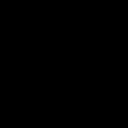
\includegraphics[scale=0.5]{imagens/black-square.png}
    \legend{Fonte:~\citeonline{tortinhas:2024}}
\end{figure}

\lipsum[1-8] % chktex-file 8


\chapter{Conclusão}%
\label{cap:conclusao}

\lipsum[1-20] % chktex-file 8

% =====

% =====
% ELEMENTOS PÓS-TEXTUAIS
% =====
% =====
% Artefatos pré-textuais
% =====

\pretextual{}

% --- Abertura ---
\insereAbertura{}

% --- Resumos ---
\begin{AmbienteResumo}
    \ValorDoConteudoDoResumo{}
\end{AmbienteResumo}
\ValorDosResumosEmLinguasEstrangeiras{}

% --- Identificação ---
\insereIndentificacao{}

% =====

% =====

\end{document}
